\section{Introduction}

With the growing popularity of data-intensive applications, the SSD density has increased rapidly in recent years.
%, expanding by 100× over the past ten years [1], [15].
As an example, in 2011, a typical 2.5-inch SSD had 256GB capacity, but
%the world's first 2TB SSD was released in 2013~\cite{foremay2013}, but 
by 2018, a high-capacity SSD boasted a 30TB, expanding by 100× over the past ten years
~\cite{samsung2011, anandtech18samsung}. 
This remarkable growth of the device-capacity is thanks to various scaling technologies 
such as nanoscale fabrication~\cite{busche2014design} and multi-layer stacking~\cite{9365809}. 
% such as nanoscale fabrication~\cite{busche2014design} and multi-layer stacking. 

% As an example, in 2011, a typical 2.5-inch SSD had 256GB capacity with 256MB of DRAM; by 2018, a high-capacity 2.5- inch SSD boasted a 30TB with 40GB of

However, not all components of the SSDs have kept up with the scaling rate.
The capacitor, which is adopted in enterprise-class SSDs for power-loss protection (PLP), fails to proceed at the pace. In general, storage devices 
have been equipped with a small size of volatile buffer. By using them for read caching and/or write buffering, they hide a long latency of the physical storage medium 
as well as mitigating an endurance limitation of the worn-out devices. 
However, the volatile buffer loses all data in the event of power crash. 
To prevent a data loss or corruption by this, enterprise-class SSDs
rely on the capacitors; it reserves energy to persist data in volatile buffer 
in the unforeseen event of a power crash. 
In addition, the adoption of capacitors enables an SSD to ignore the \texttt{FLUSH} command that explicitly requests all data in the volatile buffer to be made durable.
This property increases the buffering effect in SSD significantly, leading to both less write traffic and a shorter operation latency.

% To overcome this limitation without sacrificing performance, 
The reliance on capacitors, however, has reached its limit. 
% the improvement in capacitance fails to keep up with the rapid growth of SSDs. 
%Al(aluminum) and Ta(tantalum)-electrolytic capacitors used in SSDs have increased in density through miniaturization by tenfold from 1960 to 2005 [4]. 
Although the capacitance density has also steadily improved, 
it is not as rapid as SSD scaling speed. 
Al(aluminum) and Ta(tantalum)-electrolytic capacitors used in SSDs 
have increased in density by tenfold from 1960 to 2005,
This is approximately 50x slower than the SSD density increase rate.
Given that the internal buffer size increases in proportion to the storage capacity (typically 0.1\% of storage capacity),
the density gap between capacitance and memory technologies 
imposes an intrinsic limitation on the current architecture that 
fully protects the entire buffer data with capacitors. 


\begin{figure}[t]
    \centering{}
    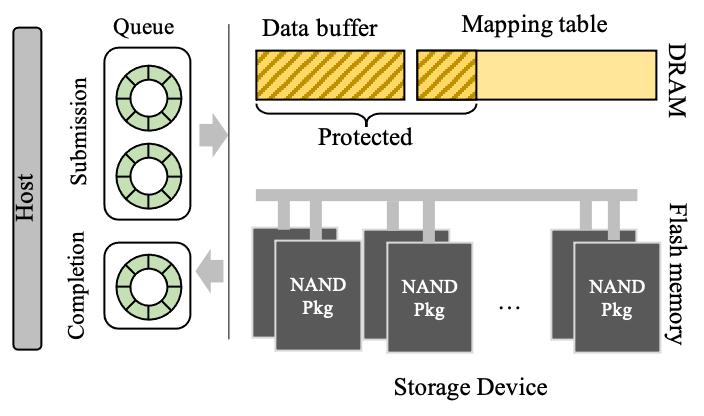
\includegraphics[width=0.4\textwidth]{figure/dawid_ssd_archi.png}
    \caption{\textbf{SSD architecture with Dawid buffer.}}
    \label{fig_spartan_archi}
\end{figure}

With this motivation, this paper presents an SSD-internal buffer architecture, called \ours{}, 
which operates under capacitance constraints. 
\ours{} essentially limits the number of dirty pages within buffer
to the level the maximum capacitance can protect.
If the number of dirty pages goes beyond the limit, they are flushed to flash memory. 
Note that the data maintained in buffer can be classified into two types: the actual user data and 
the metadata needed for their management in SSD (e.g., mapping table). 
In \ours{}, the capacitance constraint is applied only to the metadata, while protecting the user data entirely. 
This is because the storage suffers from serious performance degradation when the user data 
is not fully protected and should be entirely flushed upon a \texttt{FLUSH} command.

Based on this underlying architecture, \ours{} performs an I/O scheduling 
for the write requests within storage queue to reduce the write traffic
caused by the capacitance limitation. The scheduling algorithm aims to minimize the dirty page footprint 
of the internal buffer at a given time window. This behavior can reduce the frequency at which the number of dirty pages
exceeds the threshold and the modified pages are forced to flash memory. 
To this end, \ours{} prioritizes the write request with the least increase 
of the number of dirty pages in the mapping table.
With this policy, the write request of which the associated mapping page is already dirty 
has a top priority because it does not add the dirty page count. For other cases,  
% When the mapping page in clean state should be updated, 
\ours{} groups the write requests that modify the same mapping page 
and process them in batch in the order of group size. 
This policy enhances buffering and coalescing of the changes to the mapping table in the buffer, 
reducing a flush overhead significantly under capacitance constraints
compared to the FIFO (First-In First-Out) scheduling policy currently used in SSDs. 

To evaluate the effectiveness of \ours, we implement the proposed buffer design
in open-source SSD development framework. The performance evaluation with various workloads 
shows that \ours{} reduces the write traffic by up to 78\% and provides 25\% higher IOPS 
compared to the FIFO scheduling policy when only 10\% of the mapping table is protected. 
Compared to the full-protection architecture, \ours{} has has 20\% more writes and 
9\% of performance overhead, while reducing the required capacitance by 90\%. 

The remainder of this paper is organized as follows. In section 2, we briefly review the 
requirements and constraints for SSD with respect to reliability. Section 3 explains the 
design of SpartanSSD and Section 4 describes the implementation and performance evaluation results. 
Section 5 quantitatively analyzes the energy consumption of SSDs. Section 6 discusses our propoed design 
in relation to prior work, and Section 7 concludes. 


%define the cost for each data. the number of dirty pages increased 
% In contrast, the metadata is used only inside storage for device integrity or efficient indexing, 
% and thus it is more flexible to manage under capacitance constraints. 

%used for protecting device integrity and for accessing data 
% within storage. 

% In contrast, the metadata 
% user data 는 loss 가 발생하면 복구할 방법이 없는 반면, metadata 는 
% 사용자 데이터는 즉시 영구적으로 보호하는 것을 못한다면, 
% FLUSH command 처리에 따른 심각한 성능저하 초래. 
% host 는 반드시 flush command 를 보내야 하고, 그시점에 모든 데이터를 flush. 

% 반면 metadata 는 SSD가 해당 데이터를 잘 접근하고 SSD 자체의 integrity 유지를 위해 필요한 정보로, 
% 어느 정도 성능과 persistence 간의 

% protects user data 
%the storage buffer may be partially unprotected in power loss. 


\iffalse
\begin{itemize}
    \item capacitor density vs. SSD density 
    \item partially protected SSD 
    \item minimize the number of dirty page: write-back or management 
    \item user data cannot be managed by SSD 
    \item mapping table 의 더티 페이지 수를 줄일 수 있도록. 
\end{itemize}


A paragraph of text goes here.  Lots of text.  Plenty of interesting
text. \\

More fascinating text. Features\endnote{Remember to use endnotes, not footnotes!} galore, plethora of promises.\\
\fi